\documentclass{scrartcl}
\usepackage{amsmath}
\usepackage{hyperref}
\usepackage{graphicx}

\begin{document}
    Sources:
     \begin{itemize}
         \item \url{https://en.wikibooks.org/wiki/GLSL_Programming/Vertex_Transformations}
         \item      \url{https://developer.mozilla.org/en-US/docs/Web/API/WebGL_API/WebGL_model_view_projection}
     \end{itemize}

    \section{Transformations}

    \subsection{Modeling transformation}

        Transforms from object to world coordinates.
        \begin{itemize}
            \item Where: Vertex shader.
            \item Output: World coordinates.
            \item Output space handedness: right
            \item Transformation  matrix: \(\mathbf{M}_{\text{object}\to\text{world}}\)
        \end{itemize}


        \[
        \mathbf{M}_{\text{object}\to \text{world}} = \mathbf{A}\mathbf{t} =
        \begin{bmatrix}
            a_{1,1} & a_{1,2} & a_{1,3} & t_1 \\
            a_{2,1} & a_{2,2} & a_{2,3} & t_2 \\
            a_{3,1} & a_{3,2} & a_{3,3} & t_3 \\
            0 & 0 & 0 & 1
        \end{bmatrix}
        \]
        with $\mathbf{A}$ a matrix representing a linear transformation,
        \[
        \begin{bmatrix}
            a_{1,1} & a_{1,2} & a_{1,3} \\
            a_{2,1} & a_{2,2} & a_{2,3} \\
            a_{3,1} & a_{3,2} & a_{3,3} \\
        \end{bmatrix}
        \],
        and $\mathbf{t}$ a translation vector,
        \[
        \begin{bmatrix}
            t_1\\
            t_2\\
            t_3
        \end{bmatrix}
        \]

    If $P$ is a 3-dimensional point, we can represent it in 4-dimensional space setting the fourth coordinate to $1$:

    \[
    \begin{bmatrix}
        p_1\\
        p_2\\
        p_3 \\
        1
    \end{bmatrix}
    \]

    Then applying the affine transformation $\mathbf{M}$ to $P$ yields

    \[
    \mathbf{M}\mathbf{p} =
    \begin{bmatrix}
        a_{1,1} & a_{1,2} & a_{1,3} & t_1 \\
        a_{2,1} & a_{2,2} & a_{2,3} & t_2 \\
        a_{3,1} & a_{3,2} & a_{3,3} & t_3 \\
        0 & 0 & 0 & 1
    \end{bmatrix}
    \begin{bmatrix}
        p_1\\
        p_2\\
        p_3\\
        1
    \end{bmatrix} =
    \begin{bmatrix}
        a_{1,1}p_1 & a_{1,2}p_2 & a_{1,3}p_3 & t_1 \\
        a_{2,1}p_1 & a_{2,2}p_2 & a_{2,3}p_3 & t_2 \\
        a_{3,1}p_1 & a_{3,2}p_2 & a_{3,3}p_3 & t_3 \\
        0 & 0 & 0 & 1
    \end{bmatrix}
    \]

    which in 3d is the same as
    \[
    \mathbf{A}
    \begin{bmatrix}
        p_1\\
        p_2\\
        p_3 \\
    \end{bmatrix} +
    \begin{bmatrix}
        t_1\\
        t_2\\
        t_3
    \end{bmatrix}
    \]



    \subsection{Viewing transformation}

        Transforms from world space to view/eye space.

        \begin{itemize}
            \item Where: Vertex shader.
            \item Output: View/eye coordinates. See fig. \ref{fig:view-coordinates}
            \item Output space handedness: right
            \item Transformation matrix: \(\mathbf{M}_{\text{world}\to\text{view}}\)
        \end{itemize}


        The camera is placed at the origin of the coordinate system, points to the \textit{negative z-axis}, and sits on the\textit{ x-z plane}, with the up-direction given by the \textit{positive y-axis}.


        \begin{figure}
            \centering
            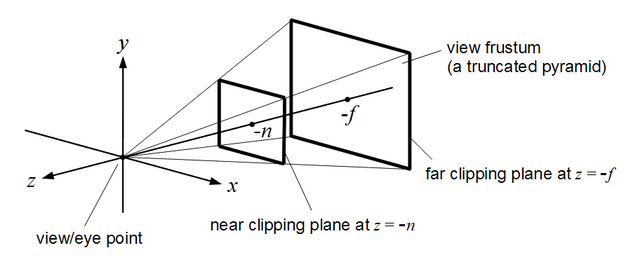
\includegraphics[width=0.8\linewidth]{view-coordinates}
            \caption{View coordinates.}
            \label{fig:view-coordinates}
        \end{figure}


        \[
        \mathbf{M}_{\text{world}\to \text{view}} =
        \begin{bmatrix}
           \mathbf{R}^T & -\mathbf{R}^T \mathbf{t} \\
            \mathbf{0}^T &1 \\
        \end{bmatrix}
        \]

        where $\mathbf{R}$ is the matrix giving the x, y, and z directions of the camera system in world coordinates

        \[
        \mathbf{R} =
        \begin{bmatrix}
           x_1 & y_1 & z_1 \\
           x_2 & y_2 & z_2 \\
           x_3 & y_3 & z_3 \\
        \end{bmatrix}
        \]

        and $\mathbf{t}$ indicates the position of the camera (again in world coordinates).

        Matrices for modeling transformation and view transformation are often combined into one \textit{ModelViewMatrix}.

    \subsection{Projection transformation}

        Transforms from camera space to clip space.

        \begin{itemize}
            \item Where: Vertex shader (e.g., outputted in \texttt{gl\_position})
            \item Output: Clip coordinates. See \ref{clip-space}.
            \item Output space handedness: left
            \item Types: orthographic and perspective.
        \end{itemize}

        \begin{figure}
            \centering
            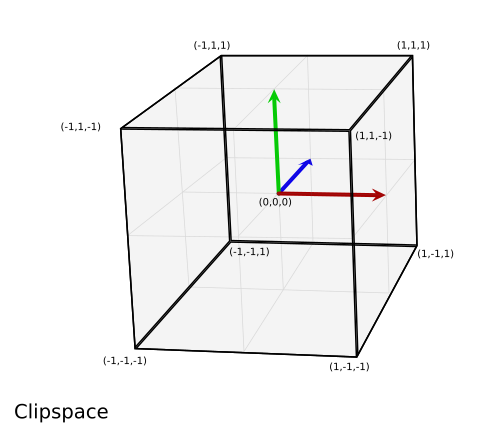
\includegraphics[width=0.8\linewidth]{clip-space}
            \caption{Clip space.}
            \label{fig:clip-space}
        \end{figure}

        Perspective projection:
        Characterized by
        \begin{itemize}
            \item an angle $\theta_{fovy}$ between x-z-plane and the y-axis
            \item the distances $n$ to the near clipping plane and $f$ to the far clipping plane
            \item  the aspect ratio $a$ of the width to the height of a centered rectangle on the near clipping plane.
        \end{itemize}
        The view point, the clipping planes, and the centered rectangle together define the view frustum, i.e. the region of 3D space that is visible for a specific projection transformation.

        \[
        \mathbf{M}_{projection} =
        \begin{bmatrix}
            \frac{d}{a} & 0 & 0 & 0 \\
            0 & a & 0 & 0 \\
            0 & 0 & \frac{n+f}{n-f} & \frac{2nf}{n-f} \\
            0 & 0 & -1 & 0
        \end{bmatrix}
        \]

        with
        \[
        d = \frac{1}{tan (\theta_{fovy}/2)}
        \]
        Here the $-1$ flips the z-axis, thus turning the coordinate system into a left-handed one.

        Orthographic projection:

        \[
        \mathbf{M}_{projection} =
        \begin{bmatrix}
            \frac{2n}{r-l} & 0 & 0 & -\frac{r+l}{r-l} \\
            0 & \frac{2}{t-b} & 0 & -\frac{t+b}{t-b} \\
            0 & 0 & \frac{-2}{f-n} & -\frac{f+n}{f-n} \\
            0 & 0 & 0 & 1
        \end{bmatrix}
        \]

        with
        \begin{itemize}
            \item n, f the distances to the clipping planes
            \item r, l, t, b the left. right, top, and bottom coordinates of the near clipping plane (at -n)
        \end{itemize}

        Here the $\frac{-2}{f-n} $ flips the z-axis, thus turning the coordinate system into a left-handed one.

    \subsection{Perspective division}

    Transforms from clip space to normalized device space (through division be the fourth coordinate, e.g., \texttt{gl\_Position.w}). This translates the 4d positions of object vertices to 3d.
    This step is done \textit{automatically} by OpenGL, since not just \texttt{gl\_Position}, but all interpolated varyings have to be transformed as well.

    \begin{itemize}
        \item Where: Between vertex shader and fragment shader (done automatically)
        \item Output: Normalized device coordinates (between -1 and 1)
        \item Output space handedness: left
    \end{itemize}

    \subsection{Viewport transformation}

    Transforms from clip space to screen space. Also done automatically by OpenGL.

    \begin{itemize}
        \item Where: fixed-function stage
        \item Output: screen coordinates
         \item Output space handedness: left
    \end{itemize}

    \[
    \mathbf{M}_{viewport} =
    \begin{bmatrix}
        \frac{w_s}{2} & 0 & 0 & s_x + \frac{w_s}{2} \\
        0 & \frac{h_s}{2} & 0 & s_y + \frac{h_s}{2} \\
        0 & 0 & \frac{f_s - n_s}{2} & \frac{f_s + n_s}{2} \\
        0 & 0 & 0 & 1
    \end{bmatrix}
    \]

    with
    \begin{itemize}
        \item $s_x$ and $s_y$ designating the lower, left corner of the viewport,
        \item $w_s$ and $h_s$ the width and height of the screen, and
        \item $n_s$ and $f_s$ the depths of the near and far clipping planes.
    \end{itemize}

\end{document}






